\documentclass[sigconf]{acmart}
\sloppy
\usepackage{graphicx}
\usepackage{color}
\settopmatter{printacmref=false} % Removes citation information below abstract
\renewcommand\footnotetextcopyrightpermission[1]{} % removes footnote with conference information in first column
\pagestyle{plain} % removes running headers
\makeatletter
\makeatother
\settopmatter{printacmref=false}

\usepackage{booktabs} % For formal tables
\setcopyright{none}

\newcommand{\MITAffiliation}{
\affiliation{%
  \institution{Massachussets Institute of Technology}
  \streetaddress{32 Vassar Street}
  \city{Cambridge}
  \state{Massachussets}
  \country{USA}
  \postcode{02139}
}}
 
 \newcommand{\EPFLAffiliation}{
\affiliation{%
  \institution{Swiss Federal Institute of Technology in Lausanne (EPFL)}
  \streetaddress{Route Cantonale}
  \city{Lausanne}
  \country{Switzerland}
  \postcode{02139}
}}

\newcommand{\srm}[1]{\textcolor{red}{{\bf Sam:} #1}}
\newcommand{\ra}[1]{\textcolor{blue}{{\bf ra:} #1}}
\newcommand{\gl}[1]{\textcolor{violet}{{\bf Gl:} #1}}
\begin{document}
\title{Learning Network Size While Training with ShrinkNets}

\author{Guillaume Leclerc, Raul Castro Fernandez, Samuel Madden}
\affiliation{%
  \institution{Massachusetts Institute of Technology}
}
\email{[leclerc, raulcf, madden]@mit.edu}

%\author{Guillaume Leclerc}
%\authornote{Visiting Student}
%\MITAffiliation
%\email{leclerc@mit.edu}
%
%\author{Raul Castro Fernandez}
%\MITAffiliation
%\email{raulcf@csail.mit.edu}
%
%\author{Samuel Madden}
%\MITAffiliation
%\email{madden@csail.mit.edu}


% The default list of authors is too long for headers.
\renewcommand{\shortauthors}{G. Leclerc et al.}


%\begin{abstract}
%  Write the abstract at the end !
%\end{abstract}

\maketitle

\section{Introduction}
Alternative intro sketch:
As neural networks become commodity in many applications from improving camera quality on mobile phones \cite{googleapple} over language translation \cite{languagetranslation} to text auto-complete \cite{autocomplete}, inference performance and model size become equally important to the quality of the prediction.  
Surprisingly, today those three concerns, quality, performance and model size, are largely handled separately with suboptimal results. 
That is, models are trained with a fixed architecture (e.g., considering a certain size and performance budget), but then during the training the network architecture is considered fixed and does not further improve.
In contrast, recently proposed techniques to make neural nets smaller after they have been trained, such as XX \cite{xx} and YY \cite{yy}, do not focus on the inference performance. 
In fact, besides universal applicable techniques such as quantitazation \cite{quant} and compiling neural networks to binary code to avoid unneccassary overhead, most existing techniques to make neural nets smaller actually harm performance as they often transform dense into sparse matrix multiplications, which is inherently slower to execute on modern hardware \cite{something}. 
%I am still not super happy with the flow. Will work on it more. 

In this paper we present a new method to automatically tune the network size while training the model to drastically improve the inference performance with comparable quality to much larger networks  
The key idea is to
\emph{learn} the right network size at the same time that the network is
learning the main task. For example, for an image classification task, with our approach we can provide the training data to a network---without sizing it a priori---and expect to end up with a network that has learned to classify images with an accuracy similar to much larger network architectures.
Our approach has two main benefits. 
First, in contrast to existing neural network compression techniques, such as brain damage, it results in small dense models, which helps to improve inference performances
Second, and most surprisingly, the resulting models are often not only much smaller but also have better accuracy than much larger models. 

Old intro:
When designing neural networks, one of the key parameters is the network size, i.e., 
%, number of layers
%and number of neuros per layer, 
%(width and depth)
the number of layers and neurons per layer.  Choosing these parameters appropriately
can dramatically affect performance, yet
%In particular, these hyper parameters have a strong correlation with
%over/underfitting \srm{give reference} \gl{I did some litterature review and
%actually this statement is quite controversial, should we rephrase ?}. 
there is no reliable way to efficiently set them. Although many search
 strategies and heuristics~\cite{Bengio2012a} have been proposed, including
%To select the best candidates, researchers have used strategies such
%as 
random search,
%\gl{Should we also move the references here if we remove the
%pargraph from the related work ?}, 
meta-gradient descent~\cite{Pedregosa2016},
Gaussian processes~\cite{Bergstra2011a}, and Parzen Estimators~\cite{Bergstra2011a}, 
%to find good parameters without exhaustively
%exploring the entire hyper-parameter space. 
 they generally require a compute-intensive
search of parameter space.

%However, we are still bound to use costly and sometimes complex methods to
%find reasonable values for these hyper-parameters.

In this paper we present a method to automatically find an appropriate network
size,
%from a single parameter, 
drastically reducing optimization time.
%dimensionality. 
The key idea is to
\emph{learn} the right network size at the same time that the network is
learning the main task. For example, for an image classification task, with our
approach we can provide the training data to a network---without sizing it a
priori---and expect to end up with a network that has learned to classify images
with an accuracy similar to a the best manually engineered network.
%\gl{too strong, we do not really have
%  any guarantee on the generalization, how about changing it to: to end up with
%  a network that learnt a tradeoff between size and accuracy}. 
Our approach has two main benefits. First, we no longer need to choose a
network size before training. Second, the final network size will tuned to be
appropriate for the task at hand, and not larger. 
%Because the sizing occurs
%dynamically, while the
%network is training, we remove the useless neurons 
%implement a new mechanism that removes
%the deactivated neurons to  
%\gl{Should we talk about the
%fact that it automatically gets rid of dead neurons ?}. 
This is important
because over-sized networks have a lower inference throughput and higher memory
footprint.

Our approach has two main challenges. First, we need a way to dynamically size the
network during training. Second, we need a loss function that optimizes
for the additional task of sizing, without deteriorating the learning
performance of the main task. Our approach, called ShrinkNets, copes with both
challenges.

% \subsection{Main Contributions}
% 
% The main contribution of this article are:
% \begin{itemize}
%   \item The Filter layer, a neural network layer which puropose is to allow feature selection
%   \item To the best of our knowledge, the first attempts to dynamically change the number of channels in deep convolutional neural networks
%   \item A deep learning library built on top of PyTorch that allow partictionners to train shrinking networks (Feed-Forward and Convolutional)
% \end{itemize}
% 

\section{ShrinkNets}

During training, our approach starts
with an explicitly over-sized network. As training progresses, we learn
which neurons are not contributing to learning and remove them
dynamically, effectively shrinking the network. This method requires two key components: first, we need a way to identify neurons that are not contributing to the
learning process, and second we need a way to balance the network size and the
generalization capability for the main task. We introduce a new \textsf{Filter} layer that takes care of \emph{deactivating} neurons. We also modify
existing loss functions to incorporate a new term that takes care of balancing
network size and generalization capability appropriately. 

%\subsection{Motivation}
%
%\srm{This makes what we have done sound like an incremental change over prior
%work.  Instead, move this description to prior work and say why its not a good
%approach there, then describe what we do as a new method.  }
%
%The method described in [ref] grows and shrinks the network over time. Though
%this seems to be an attractive property to have, during our experiments and
%according to their results, models are very slow to train and sometimes
%converge to suboptimal solutions. Their method also requires a new optimizer
%\textit{AdaRad}.  Our goal was to provide a solution that can easily be
%integrated in existing machine learning systems and provide similar convergence
%speed and accuracy. Therefore, designing a new layer that only allow shrinking
%seemed to be best approach.
%

%\subsection{Definition}

\textbf{Filter Layers: } Filter layers have weights in the range $[0,+\infty]$ and are usually placed after
linear and convolutional layers.
%\gl{This is how I
%  used it but with the new implementation we can be more creative and put them
%  anywhere, should we say "usually placed" insdead ?}. 
The \textit{Filter Layer} takes an input of size $\left(B \times C \times D_1
  \times \dots \times D_n\right)$, where $B$ is the batch size, $C$ the number
of features (or channels, in the case of convolutional layers), and $D$ any
additional dimension. This structure makes it compatible with fully connected
layers with $n=0$ or convolutional layers with $n=2$. Their crucial property is
a parameter $\theta \in \mathbb{R}^C$. The output is defined as follows: \vspace{-1em}
\begin{equation} Filter(I;\theta) = I \circ \max(0, \theta) \end{equation}
Where $\circ$ is the pointwise multiplication, and $\theta$ is expanded in all
dimensions to match the input size (except the second one since they are equal
by definition). It is easy to see that if for any $k$, if $\theta_k \leq 0$,
the $k^{\text{th}}$ input feature/channel is multiplied by zero and have no
influence on the output. If this happens, we say the Filter layer deactivates
the neuron. These disabled neurons/channels can be removed from the network
without changing its output. Before explaining how that is achieved, we explain
next how the weights of the Filter Layer are initialized and adjusted during
training.

%We can use this property to devise a training procedure.

%To train networks we need start with a substantially oversized network, then we
%insert \textit{Filter Layers}  (usually after every linear or convolutional
%layer except the last one) and we sample their weight from the
%$\text{Uniform}(0, 1)$ distribution. 

%The \textit{Filter Layer} takes an input of size $\left(B \times C \times D_1
%\times \dots \times D_n\right)$ so it is compatible with fully connected layers
%with $n=0$ or convolutional layers with $n=2$. This layer has a parameter
%$\theta \in \mathbb{R}^C$ and is defined the following way. \srm{Need to define
%B, C, D}.  
%
%\begin{equation} 
%Filter(I;\theta) = I \circ \max(0, \theta)
%\end{equation}
%
%Where $\circ$ is the Hadamard product (pointwise multiplication), and $\theta$
%is expanded in all dimensions except the second one to match the input size. It
%is easy to see that if for any $k$, if $\theta_k \leq 0$, the $k^{\text{th}}$
%feature/channel will forever be $0$. We can use this property to devise a
%training procedure.  
%
%\srm{Give an English description of what this formalism
%achieves -- what does the filter layer do, why is it significant.}

%\subsection{The training procedure}
\textbf{Training Procedure: } Once Filter layers are placed in a network and initialized (sampled from the Uniform$[0, 1]$ distribution),
%To train networks we need start with a substantially oversized network, then we
%insert \textit{Filter Layers}  (usually after every linear or convolutional
%layer except the last one) and we sample their weight from the
%$\text{Uniform}(0, 1)$ distribution. 
we could train the network directly using our standard loss function, and we could achieve performance equivalent to a normal neural
network. However, our goal is to find the smallest network with reasonable
performance. We achieve that by introducing sparsity in the parameters of the
\textit{Filter Layers}, thus forcing the deactivation of neurons%. Indeed, having a negative component in the $\theta$
%parameter of the filter layer permamently disable its associated feature
%\gl{Maybe redundant ? we talked about that in the previous paragraph} . 
. To obtain this sparsity, we simply redefine the loss function:
\vspace{-.5em}
\begin{equation}
  L'(x,y;\theta) = L(x, y) + \lambda|\max(0, \theta)|
\end{equation}

The additional term $\lambda|\max(0, \theta)|$ introduces sparsity (see Lasso
loss~\cite{Tibshirani1996}). 
% The $\lambda$ parameter, that can take any
% positive value, adjusts how aggressively the network deactivates neurons, with
% larger values indicating more aggressive deactivation.
 The second component of the loss increases the gradient with respect to $\theta$, thus pushing its value towards zero. Neurons with little impact
on the original loss (gradient lower than $\lambda$), will not be able to
compete against this attraction towards zero. Because the entries in $\theta$
with a value of $0$ or less correspond to dead neurons, $\lambda$ effectively
controls the number of neurons/channels in the entire network. We introduced
the $\max(\dots)$ into the loss to make sure that neurons are permamently disabled
when performing gradient descent based optimization. Next, we
explain how to implement ShrinkNets efficiently.

\textbf{Dynamic Network Resizing}
It is possible to reduce the overhead of the training process by removing
neurons as soon as they become deactivated by $\theta$ going to 0.
%If
%disabled neurons are not quickly removed, the overhead might cause the training
%process to be significantly slower than classic neural networks. 
To do this, we implemented a \emph{neural garbage collection} mechanism which
prunes deactivated neurons on-the-fly,  reducing the processing time
and memory overhead. To support this feature, it is crucial to understand the
information flow between neurons and layers in the neural network. We achieve
this by representing such information flow as a graph. Vertices represent layers,
and edges are event-hubs responsible for propagating information about disabled
neurons to the relevant layers.

\section{Evaluation}

We  implemented ShrinkNets, including the \emph{garbage collection}
mechanism on top of \textit{PyTorch}~\cite{paszke2017automatic}, and we have
made the software open source.\footnote{The code is available as Python/PyTorch
library on \url{http://github.com/mitdbg/fastdeepnets}
%\gl{Should we rename the repository ?}
}. We used our implementation to evaluate two crucial aspects of
ShrinkNets, which we present next.

%This is why we
%want to support what we call garbage collection: removing the weights in the
%layers that are responsible (or using) features that are disabled.  \par To be
%able to catpure this relationship between layers, we augmented \textit{Pytorch}
%~\cite{paszke2017automatic} (the framework we used as the
%foundation of our implementation) with a graph structure very similar to the
%one available in Keras ~\cite{chollet2015keras}.  In this graph, edges are
%effectively event hubs responsible for propagating \textit{feature removal}
%events to its endpoints. ShrinkNet layers are designed to emit and react to
%these events but also propagate the event further if has an impact at the other
%endpoint of the layer (input or output) \gl{What I mean here is: if the event
%  comes from the output, it might be propagated to the inputs, and the other
%  way around}.  \par This event-based implementation coordinated by edges makes
%it very easy to integrate new layers in the library.  We even provide automatic
%wrapping for layers from \textit{PyTorch} if they have no internal state. For
%more complex ones, we provide utilitaries that
%makes the implementation very concise.

%\textbf{Software architecture
%\footnote{The code is available as Python/PyTorch library on \url{http://github.com/mitdbg/fastdeepnets} \gl{Should we rename
%      the repository ?}
%}
%: }\textit{Filter Vectors} can easily be implemented in
%a few lines of code in many existing deep learning frameworks. However, in
%ShrinkNets, we assume that we start with obviously oversized networks. 
%


\subsection{Does ShrinkNet converge?}

%To demonstrate that the approach is viable, we will first show that Shrinking
%Networks converge properly. For this experiment 
We trained a one hidden layer
neural network with one filter layer to control the number of hidden units. We
initialized the models with $10000$ neurons and trained them on \texttt{MNIST}
~\cite{Lecun1998} using different values for $\lambda$.
Figure~\autoref{convergence_plot} shows that
%We
%summarized the results in \autoref{convergence_plot}. We can see on this plot
%is that for a given $\lambda$ the number of hidden units seems to always
%converge to some value. It has two implications: it seems that 
$\lambda$ works as a proxy for the network size,
% as
%we would think, a proxy of the network size 
with bigger $\lambda$ implying smaller
networks. More importantly, the figure helps us confirm that despite the regular
spikes---which are caused by the dynamic disabling of neurons---ShrinkNets
eventually converge.
%we see in the
%loss function that occur when neurons are disabled will eventually disappear
%because the number of neurons reach a plateau. 
%\gl{I feel we should give a
%  conclusion for this paragraph but I am not sure what to say}

\begin{figure}
\vspace{-.2in}
\begin{center}
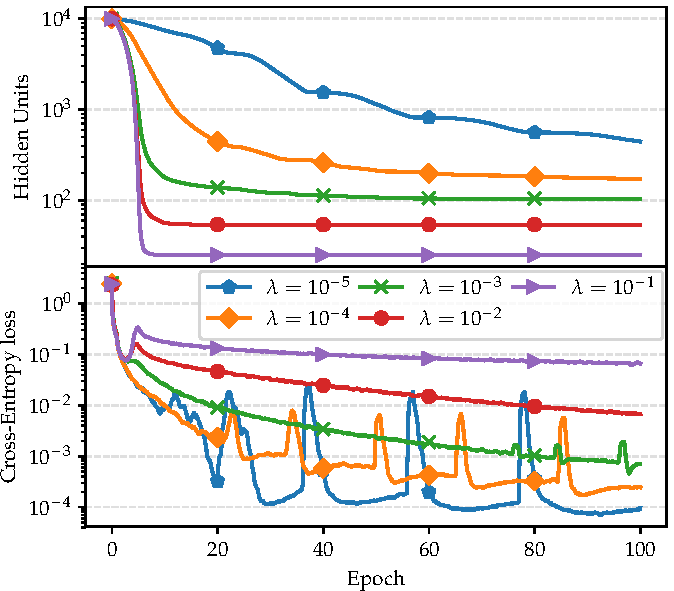
\includegraphics[width=\columnwidth]{convergence}
\vspace{-.25in}
\caption{Evolution of the number of hidden units and loss over time on the \texttt{MNIST} dataset for different $\lambda$ values \label{convergence_plot}}
\vspace{-.2in}
\end{center}
\end{figure}
\subsection{Does ShrinkNet find good networks?}

In this experiment we want to find an appropriate network size for two network
architectures, a multi-layer perceptron (MLP) and the \textit{LeNet-5}
model~\cite{Lecun1998}. We have no prior information about the network size,
but we set an upper bound of $50$ channels per convolutional layer and $5000$
neurons for fully connected layers. We then use random search to vary the
parameters that determine the network size, i.e., $\lambda$ in the case of
ShrinkNets, the width of each layer in the case of
\textsf{Fixed} and similar to previous but adding a $L_2$ penalty~\cite{Ng2004}
(\textsf{Fixed-L2}).  We train all variants on \texttt{MNIST}~\cite{Lecun1998},
\texttt{FashionMNIST}~\cite{Xiao2017} and
\texttt{CIFAR10}~\cite{Krizhevsky2009}. We use the same number of epochs, 100
for MLPs and 200 for \textit{LeNet-5}. We select the epoch that performed the
best on the validation set and evaluated it on the testing set. We repeat this
process 50 times and show the distribution of the testing accuracy in
\autoref{hyper_opt_res}.

The results in the figure show that ShrinkNets finds better networks with fewer
training iterations than the other methods, because it achieves higher median 
and less variable accuracies. Despite the simple nature of this experiment, we
believe that the results generalize to more complex search methods; mainly
because our solution reduces the dimensionality of the space they have to
explore.

%the distributions for ShrinkNets have higher
%medians and are less variable than the others. ShrinkNets can find better
%networks with fewer training iterations than the other methods
%
%We can see that in all cases the distributions for ShrinkNets have substantially
%higher medians are are less variable than the other architectures (the best
%model is not always found by ShrinkNets, but this is likely an artifact of our
%randomized search process).  This shows that ShrinkNets can find better networks
%with fewer training iterations than existing methods. 

%One of our main goals is to show that ShrinkNets quickly finds neural network
%architectures that perform well. To show this, we ran a simple experiment where
%we compare ShrinkNets to other network tuning methods, using random search over
%the hyper-parameters that control the network size ($\lambda$ in the case of
%ShrinkNets).  Despite the simple nature of this experiment, we believe that the
%results generalize to more complex search methods, many of of which will
%actually benefit dimensionality of the hyper-parameter space in the ShrinkNets
%approach.
%
%To isolate the effect of ShrinkNets we will consider two very simple
%architectures: multi-layer perceptrons (with three hidden layers) and the
%\textit{LeNet-5} model ~\cite{Lecun1998}.  For this experiment we assume we have
%no prior information about the size except an upper bound of $50$ channels per
%convolutional layer and $5000$ neurons for fully connected layers.  We try to
%find the appropriate size of the network using classical network-size
%optimization methods and ShrinkNets. For the classical methods we use: i) purely
%random selection of network size parameters (``Fixed''), as well as
%hyper-parameter regularization over the network size parameters using  $L_2$
%penalty ~\cite{Ng2004} (``Fixed-L2'').  In the experiment, 
%we randomly sample
%parameters for each class of network and  train them for the same number of
%epochs (100 for MLPs and 200 for CNNs). We picked the epoch that performed the
%best on the validation set and evaluated it on the testing set. We repeat the
%process for 50 iterations. This evaluation was done on \texttt{MNIST}
%~\cite{Lecun1998}, \texttt{FashionMNIST} ~\cite{Xiao2017} and \texttt{CIFAR10}
%~\cite{Krizhevsky2009}. The distribution of the testing accuracy we obtained is
%summarized in \autoref{hyper_opt_res}.

\begin{figure}
\vspace{-.2in}
\begin{center}
  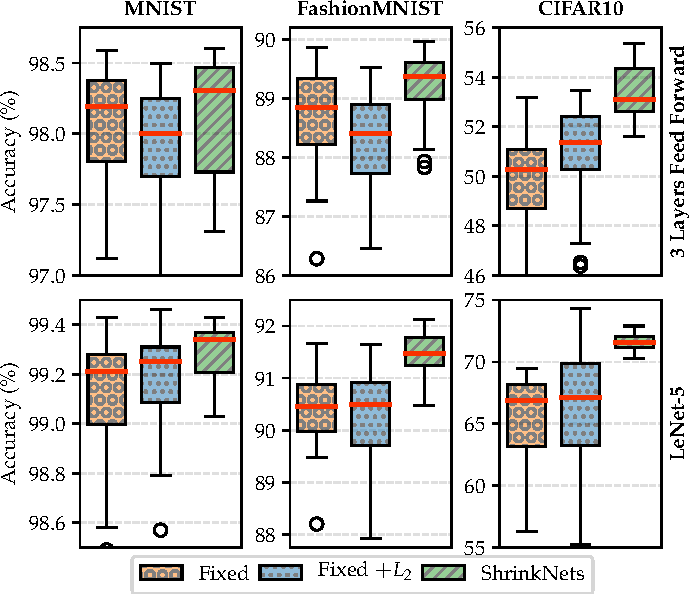
\includegraphics[width=\columnwidth]{hyper_opt}
  \vspace{-.25in}
\caption{Distributions of testing accuracy for different training methods, datasets and architectures using random search\label{hyper_opt_res}}
\vspace{-.2in}
\end{center}
\end{figure}

\section{Related Work}

There are many methods in the literature that aim to simplify network
structure. Most of them focuses on removing connections (eg: ~\cite{Cun},
~\cite{Han2015}). On the other side, ShrinkNets and some others
~\cite{Scardapane2017} and ~\cite{Philipp} try to remove entire neurons instead
of connections. This is very useful because it reduces the size of the matrices,
producing speed-up even on devices/libraries that only support dense matrices
. ShrinkNets improves on
~\cite{Scardapane2017} because it removes neurons during training, speeding up
the rest of the process. Further it outperforms~\cite{Philipp} on convergence
speed and because it does not need to change the optimizer. To the best of our
knowledge this is also the first work that tries to learn the number of channels
in a convolutional neural network.

\section{Conclusion}
In this paper we presented a novel technique to guess a
reasonable network size based on single parameter $\lambda$ that control the
tradeoff between loss and network size. We demonstrated that ShrinkNets works
both on fully connected networks and convolutional neural networks.  Although
the initial results are promising, there are many additional avenues to explore.
In the current implementation we only ``learn'' the number of features (neurons
or channels).  We plan to augment this with a dynamic number of layers as seen
in ~\cite{meier} to be able to determine the entire architecture. Further, as
shown in Figure \ref{convergence_plot} that the loss temporarily suffers from
the removal of neurons. It is likely that the loss would be more stable if the
number of neurons converged faster or neurons disappeared more slowly. For this
reason we plan to explore proximal gradient methods to optimize the filter
vectors and/or randomize neuron removals. Finally, during our evaluation we
picked small datasets mainly to be able to train many models and have
statistically significant distributions. We plan to verify that our approach see
if it generalizes to bigger datasets and other architectures like
\texttt{ResNet} ~\cite{He2016}, which is possible with small modifications to
our existing code base.

\bibliographystyle{ACM-Reference-Format}
\bibliography{bib,custom}

\end{document}
